\section{Evaluation}
\label{sec:eval}



Our evaluation is centered around an representative application: a global name service (GNS) to provide name-to-address mapping for mobile devices. 
We expect a GNS to  receive requests from clients spread in a large geographic area and the records in GNS to show a non-trivial update rate due to end-host mobility. These traits make a GNS a representative application for \auspice. In the following discussion, we refer an \auspice\ server as a \emph{name server}, an Auspice client as a \emph{local name server}, and a record as a \emph{name record} or a \emph{name}.

Our evaluation seeks to answer the following questions: (1) How well does \auspice's design meet its performance, cost, and availability goals compared to state-of-the-art alternatives under high mobility? (2) How does \auspice's cost-performance tradeoff compare to best-of-breed managed DNS services for today's (hardly mobile) domain name workloads?

\eat{Our main results are:

\begin{itemize}
\item
\emph{Lookup latency:} \auspice\ provides 5.4$\times$-11.2$\times$ lower lookup latency than \codons, a DHT-based scheme which replicates names based on popularity.
\item
\emph{Capacity:} \auspice\  sustains  a request load that is 18$\times$ the maximum load sustained by a replicate-everywhere scheme, and is comparable to the maximum load sustained by DHT-based designs.
\item
\emph{Comparison to managed DNS:} \auspice\ achieves lookup latencies comparable to a leading managed DNS provider with only one-third the locations of name resolvers. \auspice\ provides a median update latency that is 1.1 sec to 24.7 sec lower than the median update latencies of managed DNS providers.
\item
\emph{Mid-session mobility:} MSocket library enables seamless end-user mobility by migrating a TCP connection from Wi-Fi to 4G in three round trip times.
\end{itemize}
}



\vspace{-0.1in}
\subsection{Experimental setup}

\textbf{Testbeds:} We use geo-distributed testbeds (Amazon EC2 or Planetlab) or local emulation clusters (EC2 or a departmental cluster) depending upon the experiment's goals.

\textbf{Workload:} There is no real workload today of clients querying a name service in order to communicate with mobile devices frequently moving across different network addresses, both because such a name service does not exist and mobile devices do not have publicly visible IP addresses. So we conduct an evaluation using synthetic workloads for device names ($\S$\ref{sec:comparison}), but to avoid second-guessing future workload patterns, we conduct a comprehensive sensitivity analysis against all of the relevant parameters such as the read rate, write rate, popularity, and geo-locality of demand \cite{techreport}.


The following are default experimental parameters for {\em device names}. The ratio of the total number of lookups across all devices to the total number of updates is 1:1, i.e., devices are queried for on average as often as they change addresses. The lookup rate of any single device name is uniformly distributed between 0.5--1.5$\times$ the average lookup rate; the update rate is similarly distributed and drawn independently.%, so there is no correlation between the lookup and update rate of a name.


\begin{table}[t]
\centering
\small{
\begin{tabular}{c|c}
{\bf Workload parameter} & {\bf Value} \\ \hline
Fraction of (highly mobile) device names & 90\%  \\ \hline
Fraction of (mostly static) service names & 10\%   \\ \hline
\% of device name lookups   & 33.33\%  \\ \hline
\% of device name updates  & 33.33\% \\ \hline
\% of service name lookups   & 33.33\%  \\ \hline
\% of service name updates  & 0.01\% \\ \hline
Geo-locality: [devices, services] & [0.75, 0.8]  \\ \hline
\end{tabular}
}
\caption{Default workload parameters. %(except $\S$\ref{sec:sensitivity}).
}
\vspace{-0.15in}
\label{tab:setup}
\end{table}




How requests are geographically distributed is clearly important for evaluating a replica placement scheme.  We define the {\em geo-locality} of a name as the fraction of requests from the top-10\% of regions where the name is most popular. This parameter ranges from 0.1 (least locality) to 1 (high locality). For a device name with  geo-locality of $g$,  a fraction $g$ of the requests are assumed to originate from 10\% of the local name servers, the first of which is picked randomly and the rest are the ones geographically closest to it. We pick the geo-locality $g=0.75$ for device names, i.e., the top 10\% of regions in the world will account for 75\% of requests, an assumption that is consistent with the finding that communication and content access exhibits a high country-level locality \cite{twitter-www}, and is consistent with the measured geo-locality (below) of service names today.

In addition to device names, {\em service names} constitute a small fraction (10\%) of names and are intended to capture domain names like today with low mobility. Their lookup rate (or popularity) distribution and geo-distribution are used directly from the Alexa dataset \cite{alexa}. Using this dataset, we calculated the geo-locality exhibited by the top 100K websites to be 0.8. Updates for service names are a tiny fraction ($0.01\%$) of lookups as web services can be expected to be queried much more often than they are moved around. The lookup rate of service names is a third of the total number of requests (same as the lookup or update rates of devices).

Table \ref{tab:setup} summarizes the default workload parameters.


{\textbf{Replication schemes compared:}}
%\label{sec:schemes}
\textbf{\auspice} uses the replica placement strategy as described in $\S$\ref{sec:design} with the default parameter values $F=3, \mu = 0.7, \nu = 0.5$. %We set the replication control parameter ($\beta$)  to ensure that the utilization of the servers remains below  70\% (refer to Equation \ref{eq:mu}). 
We compare \auspice\ against the following: (1) \textbf{\staticthree} replicates each name at three random locations; (2) \textbf{\replicateall} replicates all names at all locations; (3) \textbf{\codons} replicates names using consistent hashing with replication similar to Codons\cite{codons-paper}. The number of replicas is chosen based on the popularity ranking of a name and  the location of replicas is decided by consistent hashing. The average hop count in Codons's underlying Beehive algorithm  is set so that it creates the same average number of replicas as \auspice\ for a fair comparison. All schemes direct a lookup to the closest available replica after the first request.

%In our implementation, each request is directly sent to the replica  that would have received this request if Pastry  routing were followed, i.e., the latency we report would be smaller than the actual latency in \codons.   We set the Zipf exponent to be $0.63$ calculated based on our workload. The average hop count is set so that \codons\ creates the same number of replicas as  \auspice\ for a fair comparison.





\vsp
\subsection{Evaluating \auspice's replica placement}
\label{sec:comparison}

We conduct experiments in this subsection on a 16-node (each with Xeon 5140, 4-cores, 8 GB RAM) departmental cluster, wherein each machine hosts 10 instances of either name servers or local name servers so as to emulate an 80-name server \auspice\ deployment. We instrument the instances so as to emulate wide-area latencies between any two instances that correspond to 160 randomly chosen Planetlab nodes. We choose emulation instead of a geo-distributed testbed in this experiment in order to obtain reproducible results while stress-testing the load-vs.-response time scaling behavior of various schemes given identical resources.

\vsp
\subsubsection{Lookup latency and update cost}
\label{sec:lookup}
\label{sec:lowload}

\begin{figure*}[t]
\centering
\subfigure[Lookup latencies (load = 0.3)]{\label{fig:namesquerymediancdf}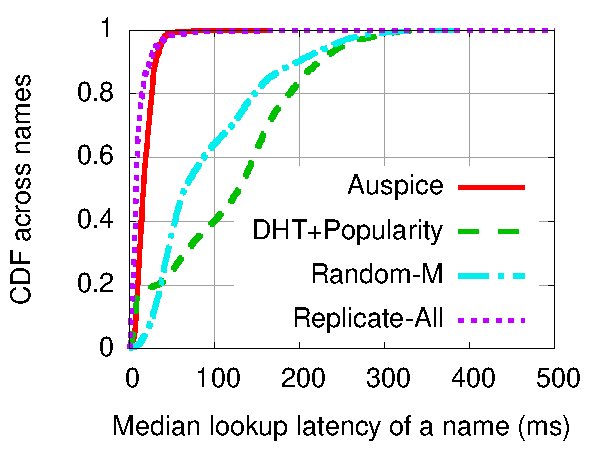
\includegraphics[scale=0.55]{graph/newgraphs/lookup-latency-cdf.pdf}}
\subfigure[Lookup latency vs. load]{\label{fig:load}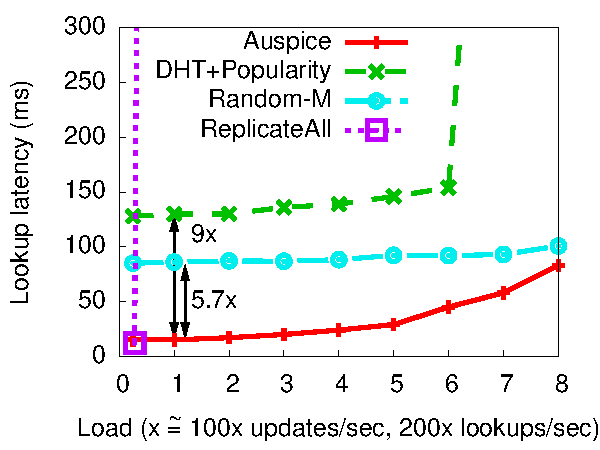
\includegraphics[scale=0.55]{graph/newgraphs/load-latency.pdf}}
\subfigure[Update cost vs. load]{\label{fig:loadupdatecost}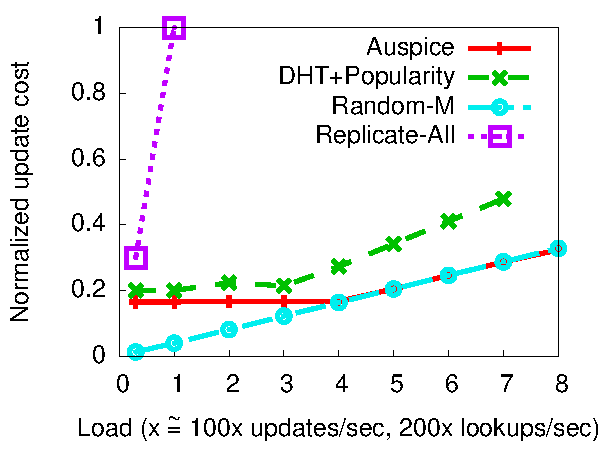
\includegraphics[scale=0.55]{graph/newgraphs/load-updatecost.pdf}}
\subfigure[Update latency]{\label{fig:updates}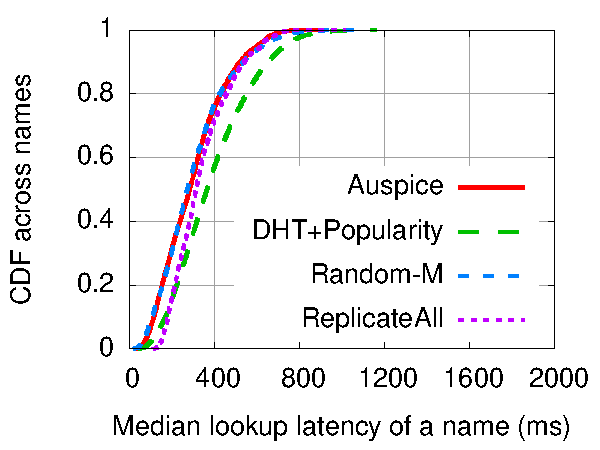
\includegraphics[scale=0.55]{graph/newgraphs/update-latency-cdf.pdf}}
\caption{\small{\auspice\ has up to 5.7$\times$ to 9$\times$ lower latencies than \staticthree\ and \codons\ reps. (\ref{fig:load}). A load of 1 means 200 lookups/sec and 100 updates/sec per name server. \replicateall\ peaks out at a load of 0.3 while \auspice\ can sustain a request load of up to 8 as it carefully chooses between 3 and 80 replicas per name. In Figure \ref{fig:updates}, median update latency of \auspice\ with total write ordering per name is 284ms and is comparable to other  schemes.}}
\vspace{-0.15in}
\label{fig:lookupupdate}
\end{figure*}

How well does \auspice\ use available resources for replicating name records? To evaluate this, we compare the lookup latency of schemes across varying load levels. A machine running 10 name servers receives on average 2000 lookups/sec and 1000 updates/sec at a load = 1. For each scheme, load is increased  until  2\% of requests fail, where a failed request means no response is received within 10 sec. The experiment runs for 10 mins for each scheme and load level. To measure steady-state behavior, both \auspice\ and \codons\ pre-compute the placement at the start of the experiment based on prior knowledge of the workload.%and retain the set of active replicas during the experiment. 

Figure \ref{fig:namesquerymediancdf} shows the distribution of median lookup latency across names at the smallest load level (load = 0.3).  Figure \ref{fig:load} shows load-vs-lookup latency curve for schemes, where ``lookup latency" refers to the mean of the median lookup latencies of names. Figure \ref{fig:loadupdatecost} shows the corresponding mean of the distribution of update cost across names at varying loads; the update cost for a name is the number of replicas times the update rate of that name.


{\em{\replicateall}}   gives low lookup latencies at the smallest load level, but generates a very high update cost and can sustain a request load of at most 0.3. This is further supported by  Figure \ref{fig:loadupdatecost} that shows that the update cost for \replicateall\ at load = 0.4 is more than the update cost of \auspice\  at load = 8. In theory, \auspice\ can have a capacity advantage of up to N/M over \replicateall, where N is the total number of name servers and M is the minimum of replicas \auspice\ must make for ensuring fault tolerance (resp. 80 and 3 here). {\em{\staticthree}} can sustain a high request load (Fig. \ref{fig:load}) due to its low update costs, but its lookup latencies are higher as it only creates 3 replicas randomly. %In theory, at low loads, \auspice\ can incur up to N/3 times more replication cost than \staticthree\ (but gain latency benefits), while at high loads, \auspice\ incurs an update cost comparable to \staticthree\ with a modest latency benefit because of better replica placement.

{\em{\auspice}}  has $5.7\times-9\times$ lower latencies over \staticthree\ and \codons\ respectively (Figure \ref{fig:load}, load=1). This is because it places a fraction of the replicas close to pockets of high demand unlike the other two.  At low to moderate loads, servers have excess capacity than the minimum needed for fault tolerance, so \auspice\ creates as many replicas as it can without exceeding the threshold utilization level (Eq. \ref{eq:mu}), thereby  achieving low latencies for loads$\leq$4. 
At loads $\geq$ 4, servers exceed the threshold utilization level even if \auspice\ creates the minimum number of replicas needed for fault tolerance. This explains why \auspice\ and \staticthree\ have equal update costs for loads $\geq$ 4 (Figure \ref{fig:loadupdatecost}). Reducing the number of replicas at higher loads allows \auspice\ to limit the update cost and sustain a maximum request load that is equal to \staticthree. 

{\em{\codons}}  has higher lookup latencies as it replicates based on lookup popularity alone and places replicas using consistent hashing without considering the geo-distribution of demand. Further, it answers lookups from a replica selected enroute the DHT route. Typically, the latency to the selected replica  is higher than the latency to the closest replica for a name, which results in high latencies.  \codons\ replicates 22.3\%   most popular names at all locations. Lookups for these names go to the closest replica and achieve low latencies; lookups for remaining 77.7\% of names incur high latencies.

\codons\  incurs higher update costs than \auspice\   even though both schemes create nearly equal numbers of replicas at every load level. This is because \codons\ decides the number of replicas of a name only based on its popularity, i.e., lookup rates, while \auspice\ decides the number of replicas based on lookup-to-update ratio of names. Due to its higher update costs, \codons\  can not sustain as high a request load as \auspice.

\vsp
\subsubsection{Update latency, update propagation delay}
\label{sec:updatelatency}

%\subfigure{\label{fig:updatelatency}\includegraphics[scale=0.55]{graph/newgraphs/}}

%This experiment evaluates the update latency of schemes.


The {\em client-perceived update latency}, i.e., the time from when when a client sends an update to when it receives a confirmation. %with total write ordering is shown in Figure \ref{fig:updates}.  
These numbers are measured from the experiment in $\S$\ref{sec:lookup} for load=0.3. The median and 90th percentile update latency for \auspice\ with total write ordering is 284ms and is comparable to other schemes. A request, after arriving an active replica, takes four one-way network delays (two rounds) to be committed by Paxos. The median update latency is a few hundred milliseconds for all schemes as it is dominated by update propagation delays.

The {\em update propagation delay}, i.e., the time from when a client issued a write till the last replica executes the write, is a key determiner of the time-to-connect. With eventual consistency, update propagation takes one round, while with total write ordering, update propagation takes two rounds and 50\% more messages.

The measured update propagation delay is consistent with expectations. With eventual consistency, this delay is 154 ms, while with total write ordering, it is 292ms. Thus. the cost of the stronger consistency provided by total write ordering compared to eventual is that it can increase the time-to-connect latency by up to 2$\times$. Note that the 2$\times$ inflation is a worst-case estimate, i.e., it will impact the time-to-connect latency only if a read request arrives at a replica while a write is under propagation to that replica, as we show below.






\subsubsection{Time-to-connect to ``moving'' endpoints}
\label{sec:ttc_exp}



We evaluate the time-to-connect to a moving destination as a function of the mobility (or update) rate.  This experiment is performed with the help of \msocket\ \cite{msocketTR}, a user-level socket library that interoperates with \auspice.  The {\em end-to-end time-to-connect}  here is measured as the latency to look up an up-to-date address of the destination (or the time-to-connect as defined in $\S$\ref{sec:design_overview}) plus the time for msocket to successfully establish a TCP connection between the client and the mobile destination. This e2e-time-to-connect also incorporates the impact of timeouts and retried lookups if the client happens to have obtained a stale value. 

The experiment is conducted on PlanetLab and consists of a single msocket client and a single mobile msocket server that is ``moving'' by changing its listening port number on a remote machine, and updating the name record replicated on three \auspice\ name servers accordingly.  A successful connection setup delay using msocket is takes 2 RTTs (2 $\times$ 105 ms)  \cite{msocketTR}.  The values of the update propagation latency $d_i$ and the lookup latency $l_i$ are 250 ms and 20 ms respectively, and the update rate $w_i$ varies from 1/1024/s to 1/s. The timeout value ($T$) in our experiment is dependent on the RTT between the client and the server. If the client attempts to connect to the server on a port which the server is not listening on, the server immediately returns an error response to the client. Specifically, the timeout value is either 1 or 2 RTTs with equal probability depending on whether the connection failed during the first or the second round-trip of msocket's connection setup.
The client sends lookups at a rate of 10/s (but this rate does not affect the time-to-connect), and both lookups and updates inter-arrival times are exponentially distributed.


Figure \ref{fig:ttc} shows the distribution of the time-to-connect with update propagation delays entailed by eventual consistency. For low-to-moderate mobility rates ($<\frac{1}{64s}$), we find that all time-to-connect values are close to 230 ms, of which 20ms is the lookup latency, and 210ms is msocket's connection setup latency. The reason the client is able to obtain the correct value upon first lookup in all cases is that the update propagation latency of 250ms is much smaller than the average inter-update interval (64s).  The update propagation delay becomes a non-trivial fraction of the inter-update interval at high mobility rates of $\approx$1/sec that results in  26\% of lookups returning stale values. The mean e2e-time-to-connect increases to  302 ms for an update rate of 1/sec, which suggests that \auspice's time-to-connect is limited by network propagation delays in this regime. Nevertheless, once a connection is successfully established, {individual} migration can quickly resynchronize the connection in $\approx$two round-trips between the client and the mobile without relying on \auspice\ (not shown here). 
%A different experiment with totally ordered writes shows qualitatively similar conclusions \cite{techreport}.

We have also developed an analytical model to predict time-to-connect values \cite{techreport}. Figure \ref{fig:ttc} also shows that the time-to-connect as predicted by our analytical model are close to those observed in the experiment, thereby re-affirming our design. 


\begin{figure*}[t]
\begin{minipage}[b]{0.48\linewidth}
\centering
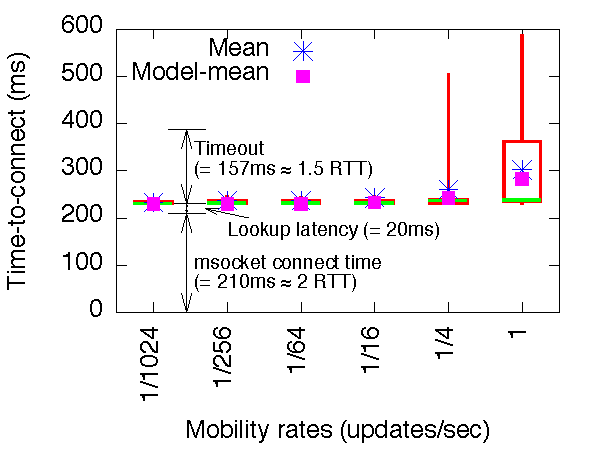
\includegraphics[scale=0.55]{graph/camera-ready/connect-time-msocket.pdf}
\caption{Time-to-connect $\approx$ lookup latency for moderate mobility rates ($<$1/100s)  as \auspice\ returns up-to-date responses w.h.p., but sharply rises thereafter.}
\label{fig:ttc}
\end{minipage}
\hspace{0.3cm}
\begin{minipage}[b]{0.48\linewidth}
\centering
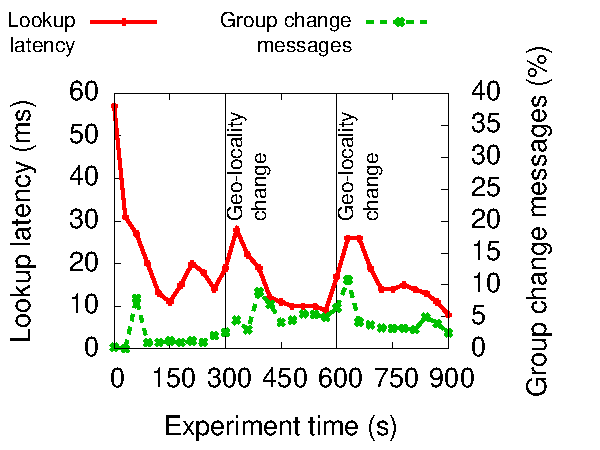
\includegraphics[scale=0.55]{graph/camera-ready/latency_by_time.pdf}
\caption{\auspice\ adapts to varying demand geo-locality in two epochs each 75s long with a (tunable) reconfiguration message overhead of 3.6\%.}
\label{fig:latency-time}
\end{minipage}
%\vspace{-0.25in}
\end{figure*}
% Box plot shows min, 5th \%-ile, median, 95th \%-ile, and max. Asterisk shows the mean.



\subsubsection{Reconfiguration overhead vs. responsiveness}

\blue{
In the next experiment, we show how \auspice\ can choose the epoch length and reconfiguration trigger so as to limit the overhead of reconfiguration (as in $\S$\ref{sec:reconf_policy}) while being responsive to changes in demand geo-locality. The workload changes the geo-distribution of demand for each name every 300 sec. 
For each name, we change the regions from which most requests arise so that changing the placement of replicas becomes necessary to minimize lookup latencies. The experiment is performed on a local cluster with a workload of 1000 names with characteristics as described in Table \ref{tab:setup}. 
The epoch length of group changes is chosen to be 75 sec, which ensures that group changes result in less than 10\% overhead to the system ($\S$\ref{sec:reconf_policy}). 
}

\blue{
We show the lookup latencies of \auspice\ and the message overhead of reconfiguration in the experiment in Figue \ref{fig:latency-time}.   We find that \auspice\ takes two epochs to infer a change in the geo-distribution of demand and to adapt to it.  This result suggests that \auspice\ can optimize lookup latencies provided the geo-distribution of demand for a name remains stable for a few epochs.
Further, we measured the overhead of reconfiguration messages in this experiment to be 3.6\%. The overhead is less than the expected overhead of 10\% because not all names are reconfigured in every epoch. 
%This finding shows that choosing epoch lengths as per the analysis in  Section \ref{sec:gc-analysis} keeps the overhead of group changes to a small fraction of the overall system load.
}



